\documentclass[]{report}

% All Dependencies

\usepackage{graphicx}
\usepackage{float}
\usepackage{amsmath}
\usepackage{amsfonts}
\usepackage{wasysym}
% Title Page
\title{MATH 4820 - Homework 2}
\author{Jack Reilly Goldrick}


\begin{document}
	\maketitle
	
	
\section{Problem 1 by Dividing the Area of Squares}
	
	\begin{itemize}
		\item Assume $\sqrt{3} = \frac{m}{n} : m > n \ \forall m,m \in \mathbb{Z}$, and m,n are co-prime
		
		\item squaring both sides and multiplying them by $n^2$ we have:
		
						$$ 3n^2 = m^2 $$
						
						
		\item Since the area of a square is the side-length squared, this equation can be interpreted as the area of the sum three squares with side-length n is equal to the area of a square with side-length m. 
		
			\begin{itemize}
				\item This implies the larger area is divisible by three, thus, we have
				
				$$ m = 3k, \forall k \in \mathbb{Z} $$
				
			\end{itemize}
			
			
			
			
			\item Substituting 2k for m we have:
			
			$$ 3n^2 = 9k^2 $$
			
			$$ n^2 = 3k^2 $$
			
			
			\begin{itemize}
				
				\item This implies that n is also divisible by three as well.
				
		\end{itemize}
		
		
		
		\item The original assumption was that these numbers m and n were co-prime to satisfy $\sqrt{3}$ as a rational number.  However, we have just shown that m and n are not co-prime for the numbers m and n to remain integers.  Thus we have raised a contradiction arising from the square root of three's rationality; therefor, the square root of three is irrational.  However, this was just to confirm that we are on the correct path.  To continue with the geometric proof we must show that the areas of every smaller sub square is also divisible by three and the infinite division is a consequence of $\sqrt{3}$'s irrationality.  Looking back on the substitution made for m with k we can see how this resulted in n being divisible by 3 as well.  Another substitution will result in showing that k is also divisible by three and so on, thus infinitely finding divisors through the same means we used prior.
		
		\item Now to show this is a consequence of irrationality, I will show what happens when we apply these ideas to any integer $k$ such that the t-root of $k$ is an integer $l$.  The reason this is the only case being considered is that any rational number with integers that do not fit this definition will be irrational due to their prime factorization and the well known fact that the $t^{th}$-root of a prime number is irrational.  Thus, any of the rationals outside the definition can be proved to be irrational in the same contradictory manner as three was considered.  Also these numbers have more than one prime fact to which is not raised to the proper exponent t. The result of having a proper exponent, t, will be shown by the same algorithm terminating in the following proof:
		
		\begin{itemize}
			
			\item Assume $\sqrt[t]{k} = \frac{m}{n} : m > n \ \forall k,l,m,n,t \in \mathbb{Z}$ with $l = \sqrt[t]{k}$, and m,n are co-prime
			
			\item Following a similar procedure we have:
			
			$$ k = \frac{m^t}{n^t} $$
			
			
			$$ km^t = n^t $$
			
			
			\item Substituting $l^t $ for $k$ we have:
			
			$$  l^{t}m^{t} = n^{t} $$
			
			
			\item This implies that $n$ is divisible by $l$ thus we have:
			
			
			$$ n = lj \ \forall j \in \mathbb{Z} $$
			
			$$  l^{t}m^{t} = l^{t}j^{t} $$
			
			$$ m^{t} = j^{t} $$ 
			
			$$ m = j $$
			
			\item Here we can se that m has no more common factors resulting in the termination of the algorithm, unlike with 3, where the algorithm kept repeating 3 as a common factor. This completes the proof that the square root of three is irrational. 
			
		\end{itemize}
		
		
		  
	\end{itemize}
	
	\begin{flushright}
		\smiley{}
	\end{flushright}
	
\section{Problem 2}

	\begin{itemize}
		\item Let $ a = 270 \land b = 168 $
		
		\item Following the Euclidean Algorithm we have:
		
		$$ 270 = q_{1}(168) + r_1  \implies q_1 = 1 \land r_1 = 102 $$ 
		
		$$ 168 = q_{2}(102) + r_2 \implies q_2 = 1 \land r_2 = 66 $$
		
		$$ 102 = q_3(66) + r_3 \implies q_3 = 1 \land r_3 = 36 $$
		
		$$ 66 = q_4(36) + r_4 \implies q_4 = 1 \land r_4 = 30 $$
		
		$$ 36 = q_5(30) + r_5 \implies q_5 = 1 \land r_5 = 6 $$
		
		$$  30 = q_6(6) + r_6 \implies q_6 = 5 \land r_6  = 0 $$
		
		
		\item This implies the gcd(270, 168) = 6
		
		\item Now to find the integer solution we have:
		\begin{align*}
		 6 &= 36 - (1 * 30)  \\
		 &= 2(36) - 66  \\		
		 &= 5(102) - 1(168)  \\
		  &= 5(270) - 6(168) 
	\end{align*}
		\item This implies $ x = 5 \land y = -6 $ 
		
	\end{itemize}
	
	
	\begin{flushright}
		\smiley{}
	\end{flushright}
	
	
	
\section{Problem 3}


	\begin{figure}[H]
		\centering
		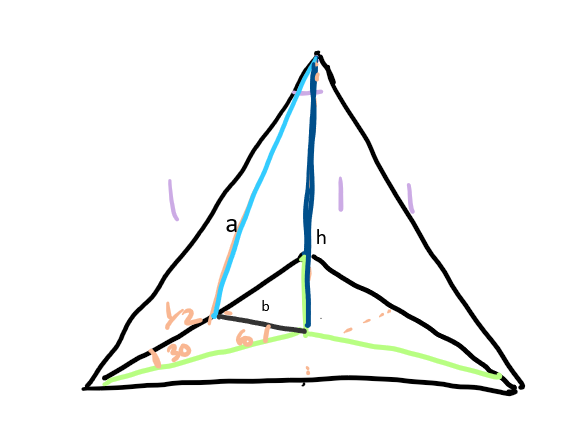
\includegraphics[width=0.7\linewidth]{pics/p3}
	\end{figure}
	
	\begin{itemize}
		\item Using my Diagram and the properties of 30-60-90 Right Triangles, we have:
		
		$$ h = \sqrt{ \frac{27}{36} - \frac{3}{36} } = \frac{\sqrt{6}}{3}  $$
	\end{itemize}

	\begin{flushright}
		\smiley{}
	\end{flushright}
	

	
	
\end{document}          
